\documentclass[11pt]{article}

\usepackage{fixltx2e}
\usepackage{amsmath}
\usepackage{amssymb}
\usepackage{amsfonts}
\usepackage[margin=1in]{geometry}
\usepackage{amsthm}
\usepackage{graphicx}
\usepackage{chngcntr}
\usepackage[section]{placeins}
\usepackage{algorithm}
\usepackage[noend]{algpseudocode}
\usepackage{amssymb}
\usepackage{mathtools}

\DeclarePairedDelimiter\ceil{\lceil}{\rceil}
\DeclarePairedDelimiter\floor{\lfloor}{\rfloor}	
	
	
\makeatletter
\def\BState{\State\hskip-\ALG@thistlm}
\makeatother

\renewcommand\thesection{\alph{section}}
\counterwithin*{section}{part}

\begin{document}
\title{Math 156 Project}
\author{Steven Yin, Fan Hin Hung}
\maketitle
\pagenumbering{gobble}
\maketitle

\pagenumbering{arabic}


\section*{Spatially spread out initial cluster centers}

\begin{figure}[h!]
\begin{minipage}{.5\textwidth}
  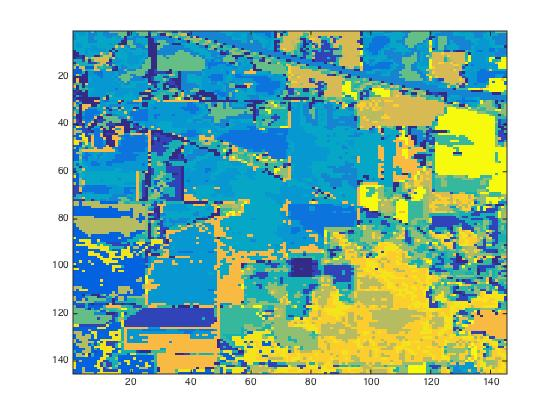
\includegraphics[scale=0.45]{init_noavg.jpg}
  \caption{Seventeen spatially spread out initial cluster centers, using raw pixel value.}
  \label{fig:3}
\end{minipage}%
\begin{minipage}{.5\textwidth}
  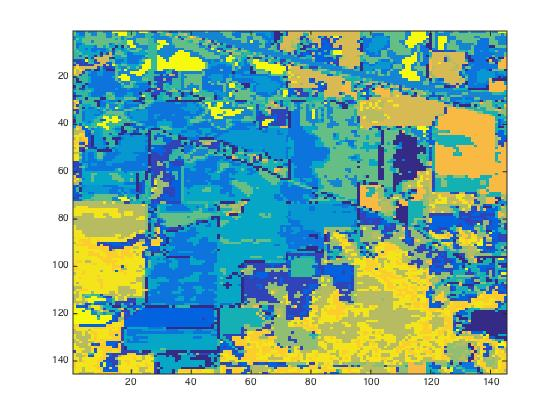
\includegraphics[scale=0.45]{init_avg.jpg}
  \caption{Seventeen spatially spread out initial cluster centers, using 5x5 averaging.}
  \label{fig:3}
\end{minipage}
\end{figure}




\section*{Plain K-means with different lambda}

\begin{figure}[h!]
\begin{minipage}{.5\textwidth}
  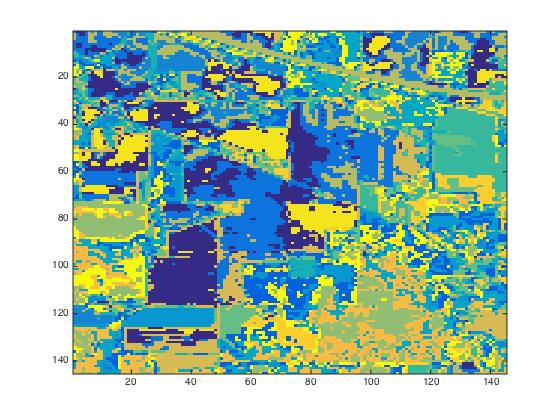
\includegraphics[scale=0.45]{plain_km_lambda10.jpg}
  \caption{$\lambda = 10$}
  \label{fig:3}
\end{minipage}%
\begin{minipage}{.5\textwidth}
  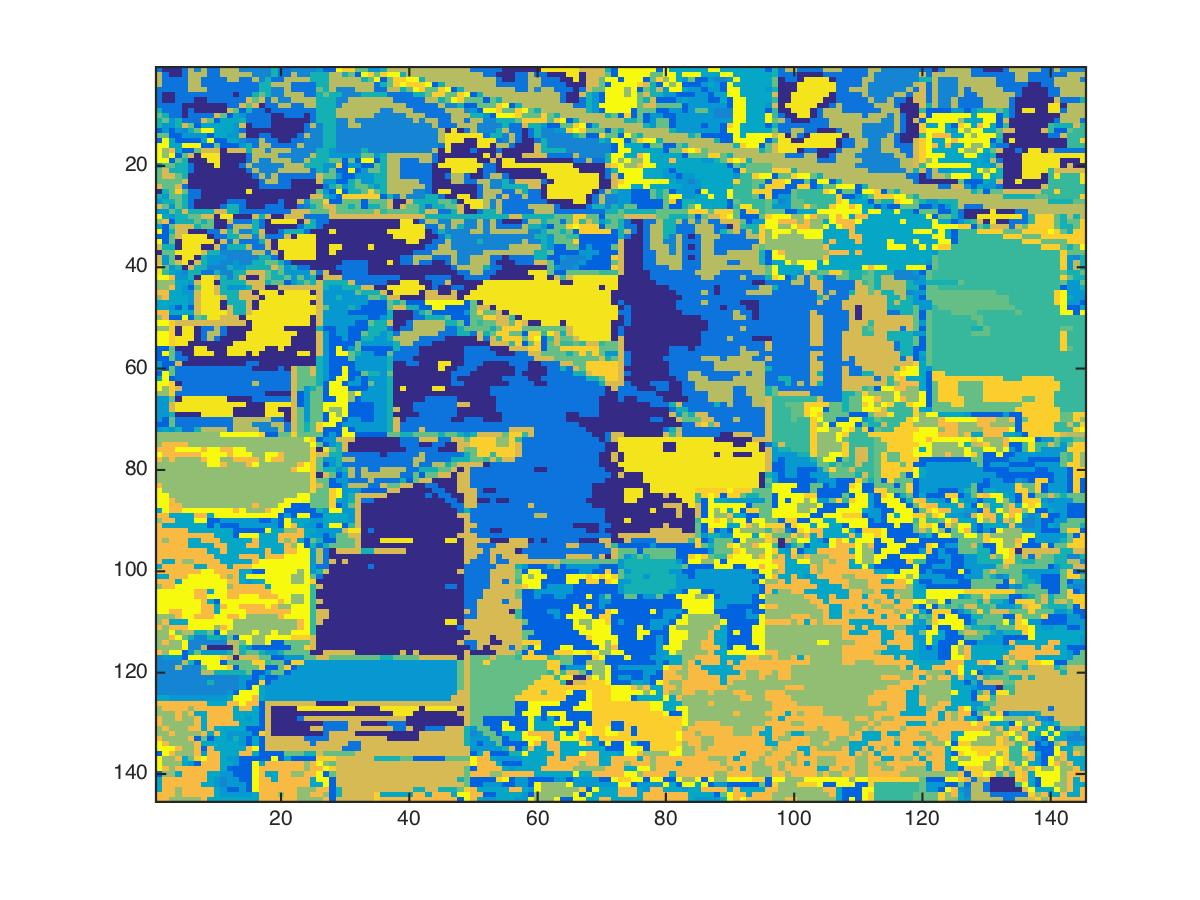
\includegraphics[scale=0.21]{plain_km_lambda25.jpg}
  \caption{$\lambda = 25$}
  \label{fig:3}
\end{minipage}
\end{figure}



\begin{figure}[h!]
\begin{minipage}{.5\textwidth}
  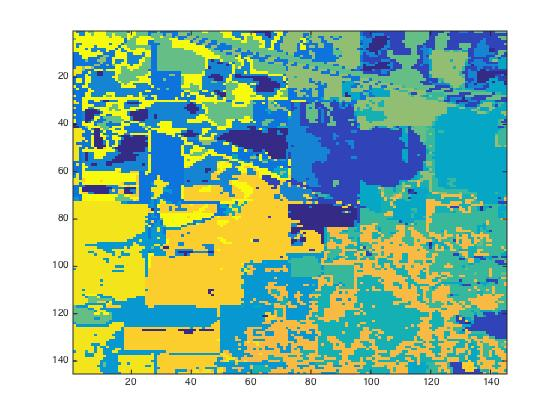
\includegraphics[scale=0.45]{plain_km_lambda50.jpg}
  \caption{$\lambda = 50$}
  \label{fig:3}
\end{minipage}%
\begin{minipage}{.5\textwidth}
  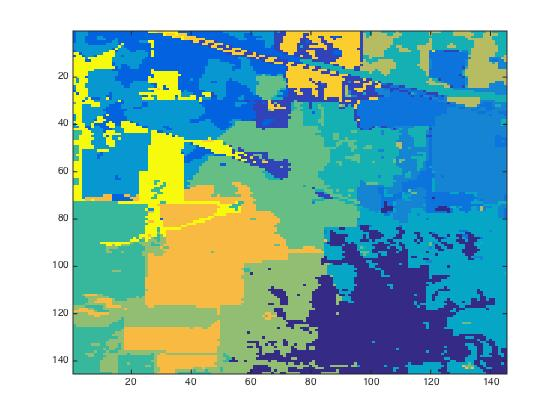
\includegraphics[scale=0.45]{plain_km_lambda100.jpg}
  \caption{$\lambda = 100$}
  \label{fig:3}
\end{minipage}
\end{figure}







\section*{Over determined means}

\begin{figure}[h!]
  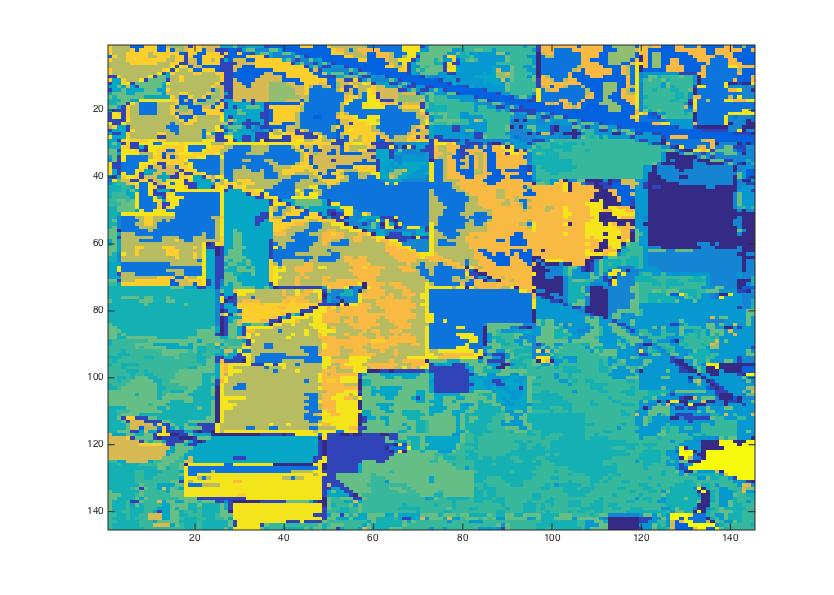
\includegraphics[scale=0.45]{km2_100cc.jpg}
  \caption{One hundred initial cluster centers.Then the cluster centers are clustered back down to 17 of them.}
  \label{fig:3}
\end{figure}








\end{document}